\documentclass[a4paper]{article}

  \usepackage{fullpage} % Package to use full page
  \usepackage{parskip} % Package to tweak paragraph skipping
  \usepackage{tikz} % Package for drawing
  \usepackage{amsmath}
  \usepackage{siunitx} % Package for scientific units
  \usepackage{amsfonts}
  \usepackage{amssymb}
  \usepackage{hyperref}
  \usepackage[utf8]{inputenc}
  \usepackage[english]{babel}
  \usepackage{multicol}
  \usepackage{graphicx} % Package for including images
  \graphicspath{ {./images/} }
  
  \newcommand\tab[1][0.5cm]{\hspace*{#1}}
  
  \title{Assignment 2}
  \author{Adrian Darian}
  \date{9/11/2020}
  
  \begin{document}
  
\maketitle
  
\section*{Chapter 2}
\begin{itemize}
	\item[6] Consider the interconnection shown in the figure below. \\
	      \hbox to 2cm{} \\	  
	      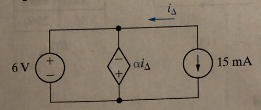
\includegraphics{P2-6.png} \\ 
	      \begin{itemize}
	      	\item[a)] What value of $\alpha$ is required to make this a valid interconnection? \\
	      	      \begin{tabular}{r c l}
	      	      	$a$ & $=$ & $\frac{\SI{-6}{\volt}}{\SI{-15}{\milli\ampere}}$ \\
	      	      	    & $=$ & $400$                                            \\
	      	      \end{tabular}
	      	\item[b)] For this value of $\alpha$, find the power associated with the current source. \\
	      	      \begin{tabular}{r c l}
	      	      	$p$ & $=$ & $\si{\volt} * i$                         \\
	      	      	    & $=$ & $\SI{6}{\volt} * \SI{15}{\milli\ampere}$ \\
	      	      	    & $=$ & $\SI{90}{\milli\watt}$                   \\
	      	      \end{tabular}
	      	\item[c)] Is the current source supplying or absorbing power? \\
	      	      absorbing
	      \end{itemize} 
	\item[9] Find the total power developed in the circuit in the figure below if $v_{o} = \SI{5}{\volt}$ \\
	      \hbox to 2cm{} \\	  
	      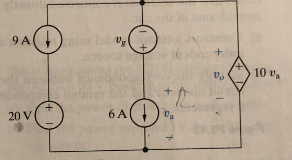
\includegraphics{P2-9.png} \\
	      \begin{tabular}{r c l}
	      	$10v_{a}$           & $=$ & $v_{o}$                                 \\
	      	$v_{a}$             & $=$ & $\SI{0.5}{\volt}$                       \\
	      	$i_{v_{a}}$         & $=$ & $\SI{15}{\ampere}$                      \\
	      	$v_{g}$             & $=$ & $v_{a} - v_{o}$                         \\
	      	                    & $=$ & $\SI{0.5}{\volt} - \SI{5}{\volt}$       \\
	      	                    & $=$ & $\SI{-4.5}{\volt}$                      \\
	      	$P_{v_{g}}$         & $=$ & $v_{g} * 6$                             \\
	      	                    & $=$ & $(-4.5) * 6$                            \\
	      	                    & $=$ & $\SI{-27}{\watt}$                       \\
	      	$v_{9_{a}}$         & $=$ & $\SI{-15}{\volt}$                       \\
	      	$P_{9\si{\ampere}}$ & $=$ & $-15 * 5$                               \\
	      	                    & $=$ & $\SI{-75}{\watt}$                       \\
	      	$P_{20\si{\volt}}$  & $=$ & $20 * 9$                                \\
	      	                    & $=$ & $\SI{180}{\watt}$                       \\
	      	$P_{v_{o}}$         & $=$ & $-(\SI{9}{\volt}) * (\SI{15}{\ampere})$ \\
	      	                    & $=$ & $\SI{-135}{\watt}$                      \\                                        
	      	$P_{total}$         & $=$ & $\SI{210}{\watt}$                       \\
	      \end{tabular}
	\item[15] A variety of current source values were applied to the device shown in the figure below \\
	      \hbox to 2cm{} \\	 
	      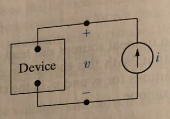
\includegraphics{P2-15.png} \\
	      \begin{tabular}{|c|c|}
	      	\hline
	      	$i\si{\milli\ampere}$ & $p\si{\milli\watt}$ \\
	      	\hline
	      	$0.5$                 & $8.25$              \\
	      	\hline
	      	$1.0$                 & $33.00$             \\
	      	\hline
	      	$1.5$                 & $74.25$             \\
	      	\hline
	      	$2.0$                 & $132.00$            \\
	      	\hline
	      	$2.5$                 & $206.25$            \\
	      	\hline
	      	$3.0$                 & $297.00$            \\
	      	\hline
	      \end{tabular}
	      \begin{itemize}
	      	\item[a)] The power absorbed by the device for each value of current is recorded in the table given in the table above. \\
	      	      \begin{tabular}{|c|c|c|}
	      	      	\hline
	      	      	$i\si{\milli\ampere}$ & $p\si{\milli\watt}$ & $R = \frac{p}{i^2}\si{\kilo\ohm}$ \\
	      	      	\hline
	      	      	$0.5$                 & $8.25$              & $33$                              \\
	      	      	\hline
	      	      	$1.0$                 & $33.00$             & $33$                              \\
	      	      	\hline
	      	      	$1.5$                 & $74.25$             & $33$                              \\
	      	      	\hline
	      	      	$2.0$                 & $132.00$            & $33$                              \\
	      	      	\hline
	      	      	$2.5$                 & $206.25$            & $33$                              \\
	      	      	\hline
	      	      	$3.0$                 & $297.00$            & $33$                              \\
	      	      	\hline
	      	      \end{tabular}
	      	\item[b)] Use the values in the table to construct a circuit model for the device consisting of a single resistor. \\
	      	      \hbox to 2cm{} \\	   
	      	      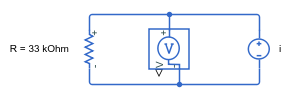
\includegraphics{circuit.png}  
	      \end{itemize}
	\item[18] Given the circuit shown in the figure below, find \\
	      \hbox to 2cm{} \\	 
	      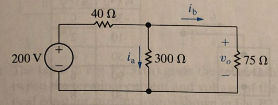
\includegraphics{P2-18.png} \\
	      \begin{itemize}
	      	\item[a)] the value of $i_{a}$ \\
	      	      \begin{tabular}{r c l}
	      	      	$i_{a}$ & $=$ & $\frac{v_{o}}{R_{a}}$ \\
	      	      	        & $=$ & $\SI{0.4}{\ampere}$   \\
	      	      \end{tabular} 
	      	\item[b)] the value of $i_{b}$ \\
	      	      \begin{tabular}{r c l}
	      	      	$i_{b}$ & $=$ & $\frac{v_{o}}{R_{b}}$ \\
	      	      	        & $=$ & $\SI{1.6}{\ampere}$   \\
	      	      \end{tabular} 
	      	\item[c)] the value of $v_{o}$ \\
	      	      \begin{tabular}{r c l}
	      	      	$\frac{v_{o} - v_{g}}{R_{g}} + \frac{v_{o}}{R_{a}} + \frac{v_{o}}{R_{b}}$ & $=$ & $0$               \\
	      	      	$\frac{v_{o} - 200}{40} + \frac{v_{o}}{300} + \frac{v_{o}}{75}$           & $=$ & $0$               \\
	      	      	$v_{o}$                                                                   & $=$ & $\SI{120}{\volt}$ \\
	      	      \end{tabular}   
	      	\item[d)] the power dissipated in each resistor \\
	      	      \begin{tabular}{r c l}
	      	      	$P_{g}$     & $=$ & $(\frac{v_{g} - v_{o}}{R_{g}})^2 * R_{g}$ \\
	      	      	            & $=$ & $\SI{160}{\watt}$                         \\
	      	      	$P_{R_{a}}$ & $=$ & $i_{a}^2 * R_{a}$                         \\
	      	      	            & $=$ & $\SI{48}{\watt}$                          \\
	      	      	$P_{R_{b}}$ & $=$ & $i_{b}^2 * R_{b}$                         \\
	      	      	            & $=$ & $\SI{192}{\watt}$                         \\
	      	      \end{tabular} 
	      	\item[e)] the power delivered by the $\SI{200}{\volt}$ source \\
	      	      \begin{tabular}{r c l}
	      	      	$P_{g}$ & $=$ & $V_{g} * I_{g}$              \\
	      	      	        & $=$ & $200 * \frac{200 - 120}{40}$ \\
	      	      	        & $=$ & $\SI{400}{\watt}$            \\
	      	      \end{tabular} 
	      \end{itemize}
	\item[24] The currents $i_{1}$ and $i_{2}$ in the circuit in the figure below are $\SI{20}{\ampere}$ and $\SI{15}{\ampere}$, respectively \\
	      \hbox to 2cm{} \\	  
	      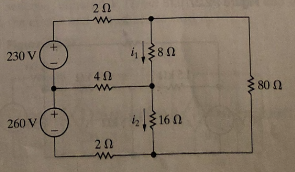
\includegraphics{P2-24.png} \\	  
	      \begin{itemize}
	      	\item[a)] Find the power supplied by each voltage source. \\
	      	      \begin{tabular}{r c l}
	      	      	$-230 + 2i_{1} + 8(i_{1} - i_{3}) + 4(i_{1} - i_{2})$  & $=$ & $0$                \\
	      	      	$-260 + 2i_{2} + 4(i_{2} - i_{1}) + 16(i_{2} - i_{3})$ & $=$ & $0$                \\
	      	      	$8(i_{3} - i_{1}) + 16(i_{3} - i_{2}) + 80i_{3}$       & $=$ & $0$                \\
	      	      	$i_{1}$                                                & $=$ & $\SI{25}{\ampere}$ \\
	      	      	$i_{2}$                                                & $=$ & $\SI{20}{\ampere}$ \\
	      	      	$i_{3}$                                                & $=$ & $\SI{5}{\ampere}$  \\
	      	      	$P_{230}$                                              & $=$ & $230i_{1}$         \\
	      	      	                                                       & $=$ & $\SI{5750}{\watt}$ \\
	      	      	$P_{260}$                                              & $=$ & $260i_{2}$         \\
	      	      	                                                       & $=$ & $\SI{5200}{\watt}$ \\
	      	      \end{tabular} 
	      	\item[b)] Show that the total power supplied equals the total power dissipated in the resistors. \\
	      	      \begin{tabular}{r c l}
	      	      	$P_{T}$ & $=$ & $P_{230} + P_{260}$                                               \\
	      	      	        & $=$ & $\SI{10,950}{\watt}$                                              \\
	      	      	$P_{d}$ & $=$ & $2i_{a} + 8i_{1} + 4(i_{a} - i_{b}) + 2i_{b} + 16i_{2} + 80i_{c}$ \\
	      	      	        & $=$ & $1250 + 3200 + 100 + 800 + 3600 + 2000$                           \\		
	      	      	        & $=$ & $\SI{10,590}{\watt}$                                              \\
	      	      \end{tabular}  
	      \end{itemize}
	\item[32] Consider the circuit shown in the figure below. \\
	      \hbox to 2cm{} \\	  
	      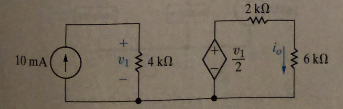
\includegraphics{P2-32.png} \\	  
	      \begin{itemize}
	      	\item[a)] Find $i_{o}$ \\
	      	      \begin{tabular}{r c l}
	      	      	$\si{\volt}_{1}$ & $=$ & $\SI{10}{\milli\ampere} * \SI{4}{\kilo\ohm}$                             \\
	      	      	                 & $=$ & $\SI{40}{\volt}$                                                         \\
	      	      	$i_{o}$          & $=$ & $\frac{\frac{\si{\volt}_{1}}{2}}{\SI{2}{\kilo\ohm} + \SI{6}{\kilo\ohm}}$ \\		
	      	      	                 & $=$ & $\SI{2.5}{\milli\ampere}$                                                \\
	      	      \end{tabular}  
	      	\item[b)] Verify the value of $i_{o}$ by showing that the power generated in the circuit equals the power absorbed in the circuit. \\
	      	      \begin{tabular}{r c l}
	      	      	$P_{generated}$ & $=$ & $\frac{\si{\volt}_{1}}{2} * \SI{2.5}{\milli\ampere}$ \\
	      	      	                & $=$ & $\SI{50}{\milli\watt}$                               \\
	      	      	$P_{absorbed}$  & $=$ & $(\SI{2}{\kilo\ohm} + \SI{6}{\kilo\ohm}) * i_{o}^2$  \\		
	      	      	                & $=$ & $\SI{50}{\milli\watt}$                               \\
	      	      \end{tabular} 
	      \end{itemize}  
\end{itemize}

  
\end{document}